\section{Theorie}
\label{sec:Theorie}

Mit der Phase eines Stoffes wird ein räumlich abgegrenzter Bereich in einem abgeschlossenen System beschrieben,
in dem sich der Stoff in einem physikalisch homogenen Zustand befindet. 
Darunter gelten unter anderem die Aggregatzustände: fest, flüssig und gasförmig.
In einem sogenannten Phasendiagramm (siehe Abbildung \ref{fig:phasendiagramm}) besitzt ein System
innerhalb eines abgegrenzten Bereichs zwei Freiheitsgrade, den Druck $p$ und die Temperatur $T$.
Das heißt, dass diese ohne Phasenänderung variiert werden können, solange keine Grenzlinie überschritten wird.

\begin{figure} 
    \centering
    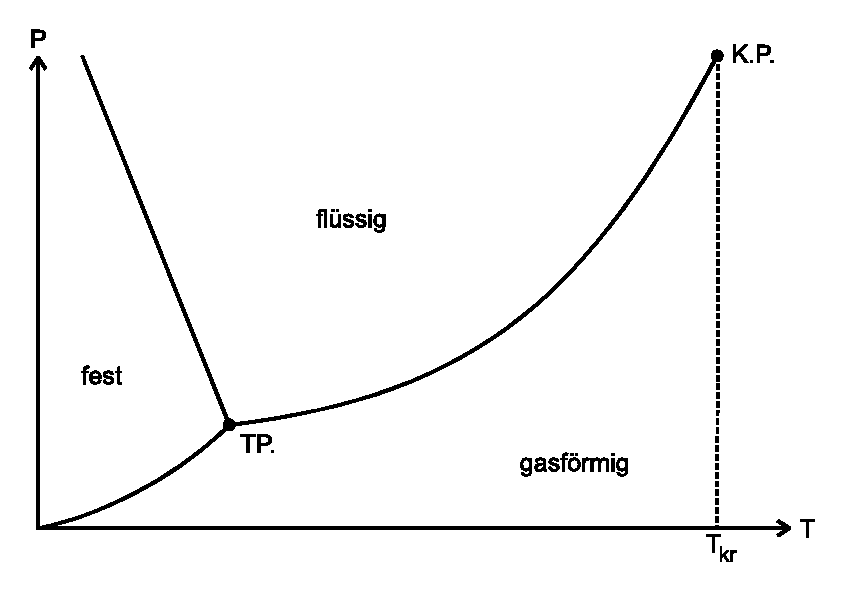
\includegraphics[width=12cm] {pictures/phasendiagramm.pdf}  
    \caption{Qualitatives Phasendiagramm von Wasser. \cite[1]{v203}}
    \label{fig:phasendiagramm}
\end{figure}

Zur Untersuchung des Übergangs von flüssig zu gasförmig, wird die Grenzlinie zwischen dem
Tripelpunkt (TP.) und den kritischen Punkt (K.P.) betrachtet, der sogenannten \textit{Dampfdruckkurve}.
An dem Tripelpunkt liegen alle drei Phasen gleichzeitig, während entlang der Kurve bis zum
kritischen Punkt die flüssige und gasförmige Phase koexistieren. \\
\\
Die Form dieser Dampfdruckkurve